\section{Machine learning model evaluation}

This chapter evaluates the predictive performance of my machine learning model.
The model's forecasts are benchmarked against both actual sensor data and the
predictions from a simpler alternative model, before discussing the results.

\subsection{Models being compared}

The three models that I compared against the actual sensor readings are included
below.

\begin{enumerate}
    \item{General forecast weather from OpenWeather} 
    \item{Proposed machine learning model (Chapter \ref{sec:machine-learning})} 
    \item{Alternative model - an adjusted version of the OpenWeather using a mean average adjustment}
\end{enumerate}

\subsection{Procedure}

To evaluate the models I compared the results from all three models over the
same 48 hour period (which is the limit of the OpenWeather forecast). The
measurements started at 00:00 on Saturday, 30 August 2025, and concluded at
23:00 on Sunday, 31 August 2025. 

The OpenWeather forecast and machine learning prediction were collected
automatically by my backend (using node\_cron and endpoints, see Section
\ref{sec:building-api}) and stored in a temporary database table I made
specifically for this evaluation.

The alternative model was made by comparing the average temperature, humidity
and wind speed differences between my raw sensor data and OpenWeather current
weather readings from my database. An average difference was then calculated
between the two datasets and applied to the raw OpenWeather forecast. The aim of
this was to adjust the forecast readings to be closer to the sensor readings. To
make the comparison fair with the machine learning model, I used data from
15--27 August (the same as the ML's training data) so that the alternative model
would not have a larger amount of data. The purpose of including the alternative
model was to assess whether a simple bias correction model was any different to
my more complex machine learning procedure.

\subsection{Charts and results}

As the weather data for the selected period was very similar between both nodes
I have decided to only show charts for node 1 as it is representative of node 2
as well. I have included a table containing the Mean Absolute Error (MAE) and
Root Mean Squared Error (RMSE) for the data in these charts in Appendix
\ref{app:ml-stats}.

\begin{figure}[H]
    \centering
    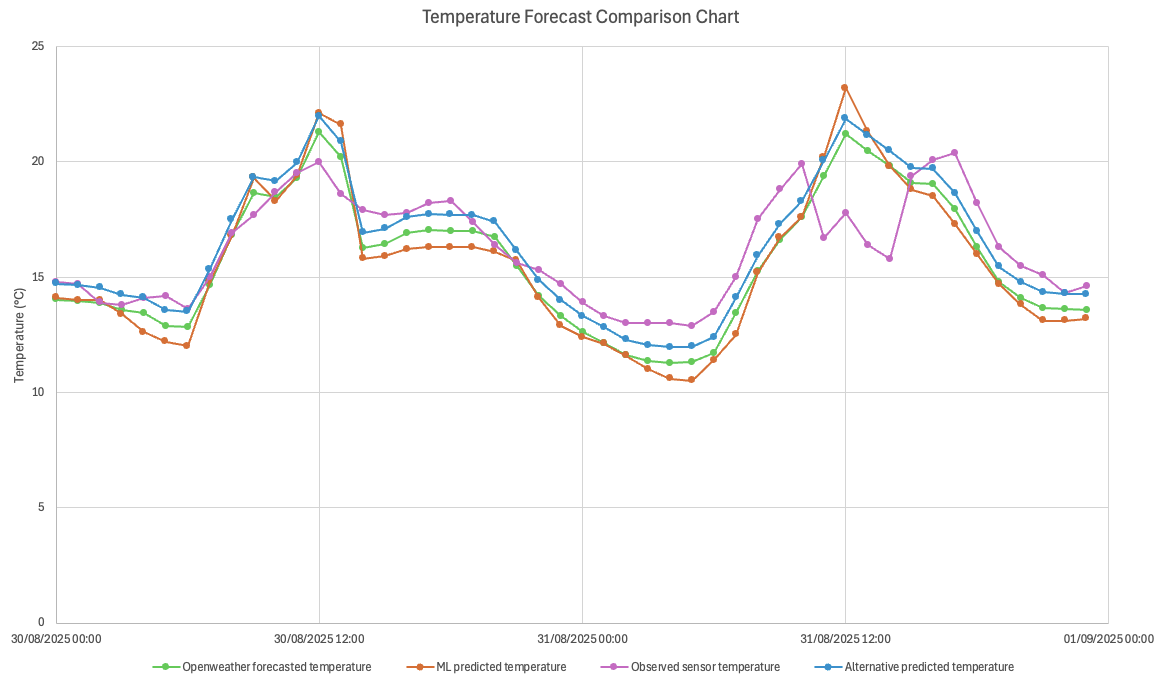
\includegraphics[width=0.95\textwidth]{contents/part-4/fig4/temperature-graph.png}
    \caption{Chart comparing temperature forecast models}
    \label{fig:temperature-chart}
\end{figure}

While Figure \ref{fig:temperature-chart} does show that the machine learning
model (orange) roughly tracked the observed readings, it does not appear to be
substantially more accurate than either the general forecast (green) or the
alternative model (blue). The relative MAE (see Appendix \ref{app:ml-stats}) of
the machine learning model here is 2.9\% while the general forecast is only
slightly higher at 3.4\%\footnote{MAE scores should be interpreted as follows: a
higher score means that the error compared to the actual sensor reading was
greater. A lower score indicates a closer (better) relationship}, meaning the ML
model is only marginally better than its input data at predicting temperature.
The alternative model performs better with an MAE of 1.3\%. Both the ML and
alternative models predicted a higher peak temperature on both days than either
the sensor data or the forecast, suggesting that the data from 15th - 27th
August may not have been a representative sample and is biased towards higher
temperatures.

\begin{figure}[H]
    \centering
    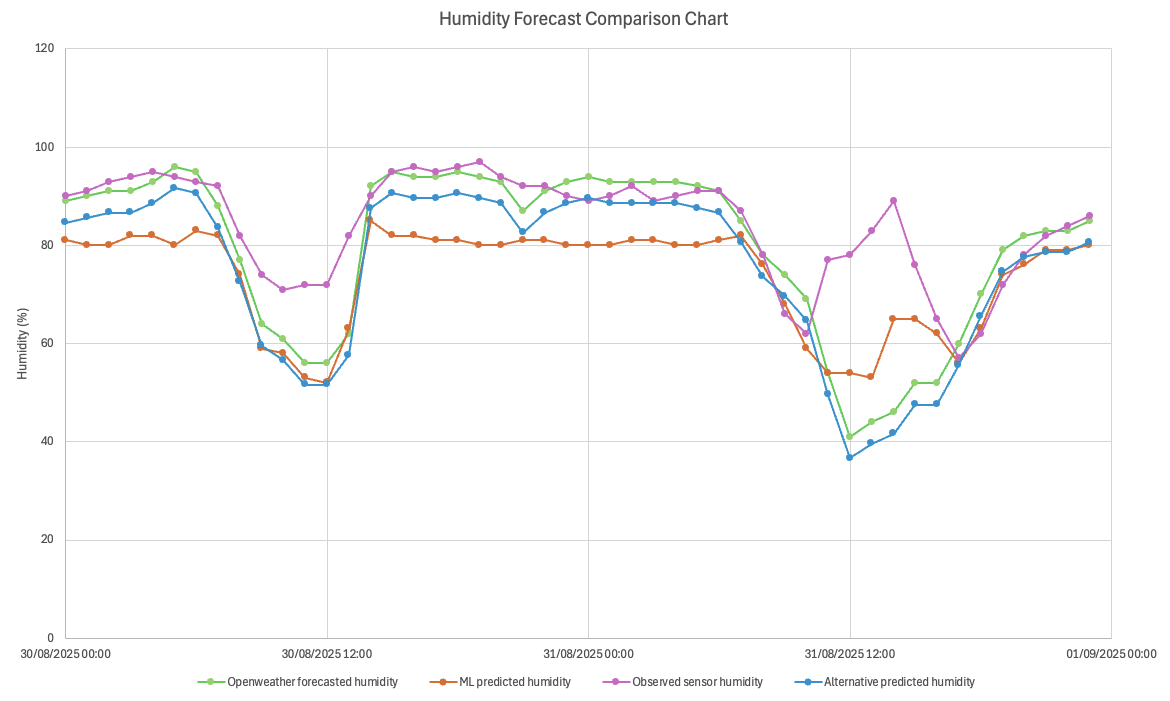
\includegraphics[width=1\textwidth]{contents/part-4/fig4/humidity-graph.png}
    \caption{Chart comparing humidity forecast models}
    \label{fig:humidity-chart}
\end{figure}

In Figure \ref{fig:humidity-chart} the machine learning model performed
particularly poorly on average with an MAE OF 14.9\% (General forecast: 5.5\%).
The alternative model also performs worse with MAE of 11.1\%. While these
metrics paint a poor picture of the model, I would point to the section of the
chart around 12:00 31/08. Here we can see that the machine learning model is the
only one of the models to successfully predict a spike in humidity at midday.
While the magnitude of this spike is not correct it does offer some tentative
evidence that the model can more accurately predict some data patterns that a
the general forecasts cannot predict.

\begin{figure}[H]
    \centering
    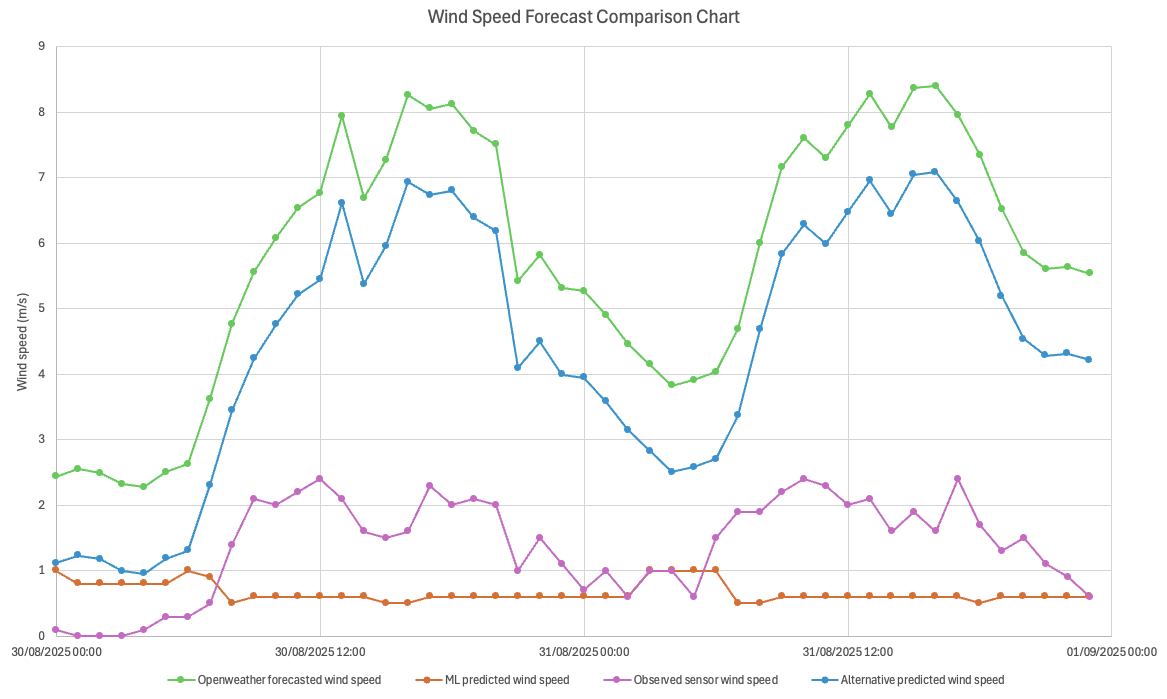
\includegraphics[width=1\textwidth]{contents/part-4/fig4/wind-speed-graph.png}
    \caption{Chart comparing wind speed forecast models}
    \label{fig:wind-chart}
\end{figure}

With wind speed (Figure \ref{fig:wind-chart}) the ML model performs better
relative to either the general forecast or the adjusted forecast used in the
alternative model. This is reflected in an MAE of 43.6\% for the machine
learning model versus 381.9\% and 264\% for the general forecast and alternative
model respectively. With that said, the machine learning model does not show any
"hump" at midday meaning that the model is not predicting the pattern of wind
speed well. This suggests the training data had fewer windy days than the 48
hours evaluated here

\begin{figure}[H]
    \centering
    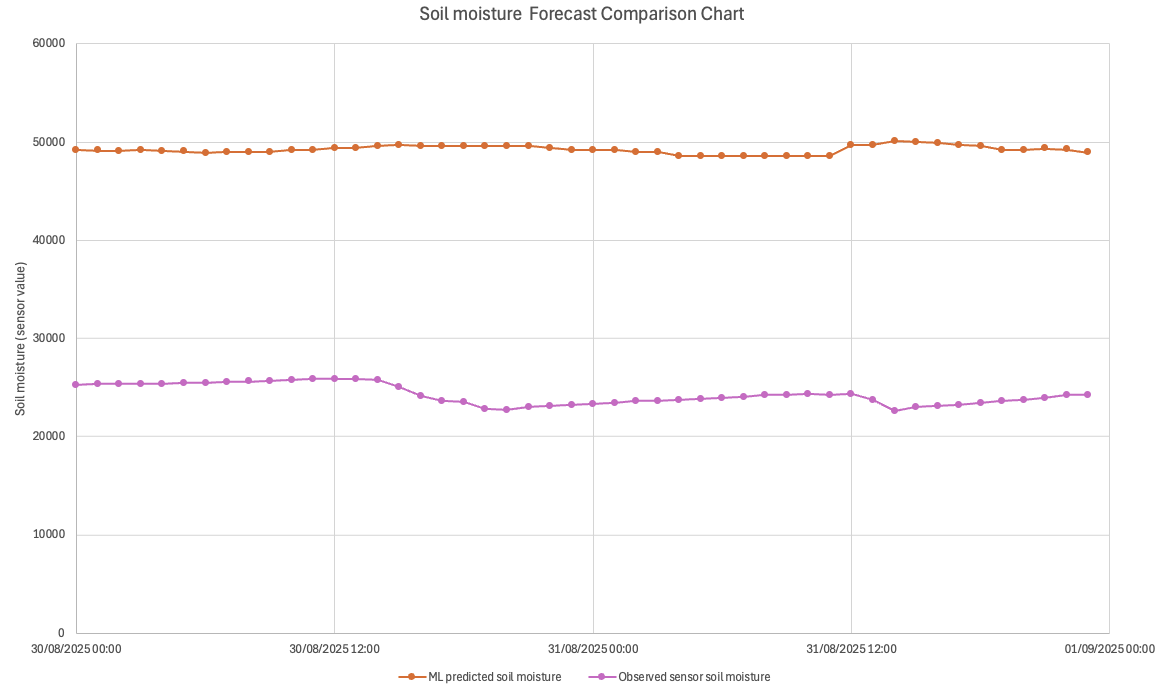
\includegraphics[width=1\textwidth]{contents/part-4/fig4/soil-graph.png}
    \caption{Chart comparing soil moisture predicted by machine learning model versus actual readings}
    \label{fig:soil-chart}
\end{figure}

The soil moisture chart (Figure \ref{fig:wind-chart}) only has the data for the
machine learning model and the observed data because the general forecast and
alternative models do not capture this metric. The large MAE of 162\% here is
not surprising at all however - the model's training data was all from an
extremely dry period of time and therefore the model does not adjust soil
moisture for recent precipitation. The days before the 48 hour period used in
these charts had included a lot of rain so the soil was still still wet from
this. However the model still expected dry soil as no connection between
rainfall and damp soil had been established in the training rounds.

\subsection{Discussion of results}

While the results for the machine learning model are mixed, there are some
bright spots. For example, the model still broadly tracks the actual sensor
readings for both temperature and humidity. With respect to temperature, while
the MAE of 2.9\% was not the best score, in Celsius this represents an error of
less than 0.5$^\circ$C. If we only look at the temperature error for node~2, the
error was even smaller at around 0.2$^\circ$C (node~1 was 0.7$^\circ$C), and it
was the best performer of the three in this context.

Additionally, the humidity chart shows that the model can detect some patterns
that the general forecast does not, as seen in the brief reversal in humidity on
day~2. Wind speed and soil moisture were clear wins for the model, but mostly
due to the highly inflated figures for wind in the forecast and the lack of any
soil moisture forecast data.

Despite this, on average the alternative model marginally outperformed the
machine learning model in temperature, and both models were surprisingly worse
than the general forecast in the humidity context. This raises the question of
whether machine learning is "worth it" if a computationally simpler model
performed at around the same level.

I would argue that yes, using machine learning was worth it, for two reasons:
The first is around the training data: the machine learning model here was not
trained on nearly enough data to provide a fair evaluation of its
microforecasting abilities compared to the other models. This is most obvious
from the soil moisture readings, where the model had no prior rain data meaning
it would have been impossible to predict that soil moisture levels would be
lower after rainfall. In general weather conditions from the 15th to the 27th
are not particularly representative of the conditions after this point, as the
weather has been cooler and cloudier past this point with higher average
humidity.

The second point is that the machine learning approach is capable and likely to
improve, unlike the other solutions which are fundamentally not predicting the
microclimate. For example the alternative model is essentially a blunt
correction to the general forecast, as the dataset grows this approach would
become increasingly poor. If in summer the microclimate tends to be hotter and
in winter it tends to be cooler then using a simple mean average correction
would not only result in no change to the forecast but also a poor prediction in
both seasons.

Hence I believe that with a longer deployment and more data it is highly likely
that the machine learning approach would show much greater accuracy than the
other approaches, and is one of the interesting avenues for future work (Section
\ref{sec:future-work}).